\documentclass[10pt, conference, compsocconf]{llncs}
% Add the compsocconf option for Computer Society conferences.
%
% If IEEEtran.cls has not been installed into the LaTeX system files,
% manually specify the path to it like:
% \documentclass[conference]{../sty/IEEEtran}
\newcommand{\highlight}[1]{\colorbox{yellow}{#1}}


% Some very useful LaTeX packages include:

% *** MISC UTILITY PACKAGES ***
%
\usepackage{ifpdf}


% *** CITATION PACKAGES ***
%
%\usepackage{cite}


% *** MATH PACKAGES ***
%
\usepackage[cmex10]{amsmath}
\usepackage{amssymb}

% *** SPECIALIZED LIST PACKAGES ***
%
\usepackage{algorithmic}


% *** ALIGNMENT PACKAGES ***
%
\usepackage{array}

% *** SUBFIGURE PACKAGES ***
%
\usepackage[tight,footnotesize]{subfigure}

% *** FLOAT PACKAGES ***
%
\usepackage{fixltx2e}
\usepackage{stfloats}

% *** GRAPHICS PACKAGES ***
%
\usepackage{graphicx}

% *** BIBLIOGRAPHY PACKAGES ***
%
\usepackage{natbib}

% *** LANGUAGE PACKAGES ***
%
\usepackage[utf8]{inputenc} 
\usepackage[T1]{fontenc}      
\usepackage[french]{babel}

% *** LAYOUT PACKAGES ***
%
\usepackage[top=4cm, bottom=4cm, left=4cm, right=4cm]{geometry}


\begin{document}
%
% paper title
% can use linebreaks \\ within to get better formatting as desired
\title{Les Citizen Sciences dans\\l'accomplissement des SDGs : \\un exemple environnemental}





% author names and affiliations
% use a multiple column layout for up to two different
% affiliations
% 
\author{Djavan Sergent \\
Master en Sciences Informatiques \\
djavan.sergent@etu.unige.ch}

\institute{Université de Genève}



% make the title area
\maketitle


\begin{abstract}
	<ABSTRACT>
\end{abstract}


\textbf{Mots clés} Citizen Science ; Monitoring ; Water Quality ; Sustainable Development


\section{Introduction}
	En 2000, les Nations-Unies lancent le programme des Millenim Developpment Goals (MDGs) qui s'étend jusq'en 2015 \cite{united_nations_millennium_2009}. Il s'agit d'un ensemble d'objectifs internationaux parmi lesquels on peut notamment citer l'éradication de l'extrême pauvreté et de la faim, combattre la mortalité infantile ou encore apporter une éducation à toutes et tous. Les 191 états membres des Nations-Unies ainsi que 22 organisations internationnales se sont engagées à participer activement à la réalisation de ces objectifs \cite{wikipedia_millennium_2017}.
	
	Fin 2015, beaucoup d'efforts ont été investis, mais les progrès sont encore très inégaux. Les différents pays membres des Nations-Unies ainsi que des organisations civiles se sont donc intéressées à l'agenda post-2015, c'est à dire aux objectifs futurs. Les Sustainable Developpment Goals (SDGs) ont étés acceptés comme relève des MDGs \cite{wikipedia_sustainable_2017}. Ceux-ci comportent 17 buts, chacuns subdivisé en objectifs. Les SDGs totalisent 169 objectifs qui possédent tous leurs propres indicateurs.
	\begin{figure}
		\begin{center}
			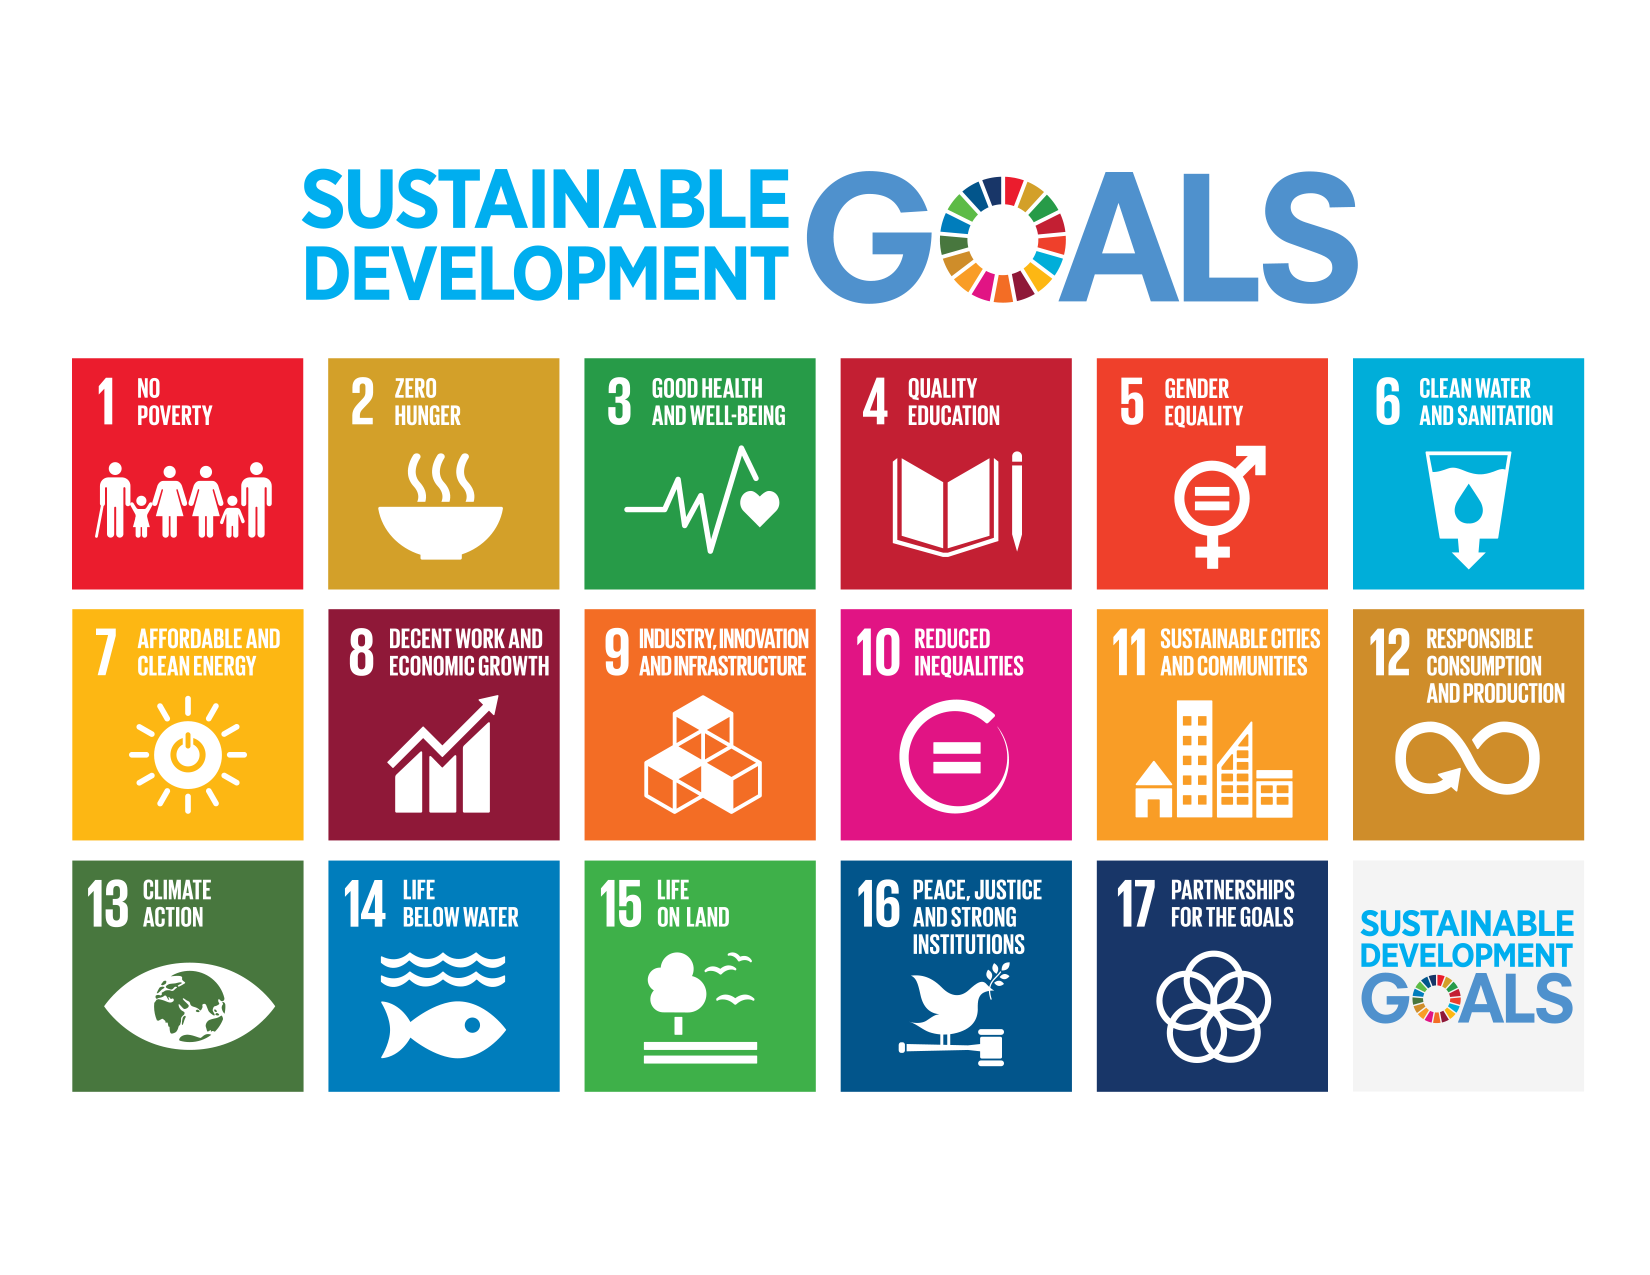
\includegraphics[width=300pt]{sdgs.png}
		\end{center}
		\caption{Icônes des SDGs (source : Sustainable Development Knowledge Platform)}
	\end{figure}
	\\
	Nous analysons dans cet article le rôle du numérique dans la réalisation des certains SDGs, particulièrement du point de vue de la participation citoyenne. Une attention spéciale est portée sur la qualité de l'eau et de l'air, sur les différents indicateurs qui permettent de l'évaluer et sur les méthodes de surveillance utilisé tant au niveau global, par exemple par satellite, que local au moyen de prélèvements.

\section{Sustainable Developpment Goals}
		\subsection{Objectifs}
			Nous nous intéressons, dans le cadre de cet article, aux buts décrits ci-dessous. Il est cependant important de noter que les objectifs sont intrinséquement liés entre eux et s'influencent mutuellement. Par exemple, en formant des citoyens à l'utilisation de matériel de mesure de qualité de l'eau, on va agir non seulement sur la capacité à, entre autre, détecter la pollution mais également sur l'éducation.
			\begin{description}
				\item[ 3 - Good Health and Well-Being :] La santé et la pollution de l'air sont au centre de ce but.
				\item[ 6 - Clean water and sanitation :] Un accès universel à l'eau et aux installations sanitaires est essentiel pour la santé humaine, la prospérité économique et la préservation de l'environnement.
				\item[14 - Life below water :] L'acidification des océans, la surpêche ou encore la pollution marine ont un impact important sur la protection des océans. Leur dégradation provoque des effets sur certaines espèces marines mais également sur la biodiversité et le fonctionnement des écosystèmes.
			\end{description}				
		
		\subsection{Progrès, revue et indicateurs}
			Le High-Level Political Forum (HLPF), créé en 2012 à la suite de Rio20+, est chargé de promouvoir les objectifs, d'assurer un suivi et d'émettre des recommandations pour la réalisation des SDGs. Ce forum se réunit annuellement. \\
			Les dix-sept buts possèdent leurs propres indicateurs globaux et standardisés. Ces indicateurs servent à évaluer les progrès effectués au niveau international, national, régional et local. \\
			Le HLPF revoit une partie des objectifs lors des réunions annuelles, les autres sont abordés à une session ultérieure. La participation et la collaboration est revue chaque année pour favoriser le développement des SDGs.

\section{Monitoring environnemental}
	\subsection{Eau}
			L'eau est l'une des ressources naturelles les plus importante sur terre. Elle joue un rôle essentiel dans de multiples secteurs économiques, sanitaires et environnementaux.\\
			L'accès à l'eau potable, à des installations sanitaires et un plan de gestion des ressources est un enjeu majeur des SDGs. Réparties de façon inégale sur terre % \cite{lefevre_repartition_nodate}
			, l'eau est essentielle pour le développement économique, l'agriculture, la protection de l'environnement ou encore la santé. Dans de nombreux pays tels que les États-Unis, la plus grande partie de cette eau est dédiée à l'agriculture %\cite{world_business_council_for_sustainable_development_global_nodate}.
			Dans ce contexte, il est important de mettre en oeuvre des systèmes de gestion des ressources hydriques et de permettre un accès universel à des sources d'eau propre. Ce but a un impact sur d'autres tels que la santé ou la lutte contre la faim.\\
			Selon les rapports du secrétaire-général du conseil économique et social des Nations-Unies \cite{united_nations_economic_and_social_council_progress_2017}\cite{united_nations_economic_and_social_council_progress_2017-1}, un tiers de la population mondiale n'a, en 2015, pas accès à des installations sanitaires. Selon les même rapports, parmi eux, 946 millions n'ont accès à aucune infrastructure. La mauvaise gestion des déchêts humains représente un risque concret pour la santé et pour l'environnement \cite{ashbolt_microbial_2004}.\\
			Concernant l'accès à l'eau potable, la situation évolue positivement. On constate qu'en 2000, 82 pourcent de la population dispose d'une source d'eau aménagée contre 91\% en 2015. Cependant, on estime également qu'environ 25\% de la population mondiale est exposée à de l'eau contaminée par des matières fécales \cite{united_nations_goal_nodate-4}. \\
			Selon le rapport \cite{rana_water_2017}, il n'existe pas de plan complet qui permette la mise en place d'un système de gestion renouvelable des ressources en eau et le manque de données précises rend impossible l'évaluation des performances pour les approches actuellement implémentées. \\
			Toujours d'après ce même rapport, les innondations sont à l'origine de nombreuses maladies et dommages causés à des infrastructures. Les innondations peuvent causer des épidémies, comme le démontre le cas de Itaparica Dam au Brésil lors duquel, en 1988, plus de 2000 cas de gastroantérite sont déclarés sur une période de 42 jours. 88 d'entre eux s'avéreront mortels. Les innondations favorisent également la reproduction des moustiques et ainsi la propagation de maladies telles que la Rift Valley Fever (RFV) \cite{hanafi_rift_2010}.\\
			Un aspect également très important de la gestion de l'eau concerne les "Dead Zones" qui s'étendent de façon exponnentielle depuis 1960 \cite{diaz_spreading_2008}. Les "Dead Zones" sont de larges étendues d'eau qui n'ont plus assez d'oxygène pour assurer la vie marine. En 2008, 400 de ces zones affectant plus de 245'000km$^{2}$, majoritairement situées dans les océans, sont répertoriées. La cause principale du développement des "Dead Zones" est la libération dans l'eau de nutriments qui accélèrent la croissance de certaines algues, réduisant la quantité d'oxygène disponible sous la surface. Bien que ces zones soient souvent d'origine naturelle, leur croissance est particulièrement accélérée par la proximité de sites industriels et agricoles qui rejettent leurs nutriments dans l'eau. \\
			\begin{figure}
				\begin{center}
					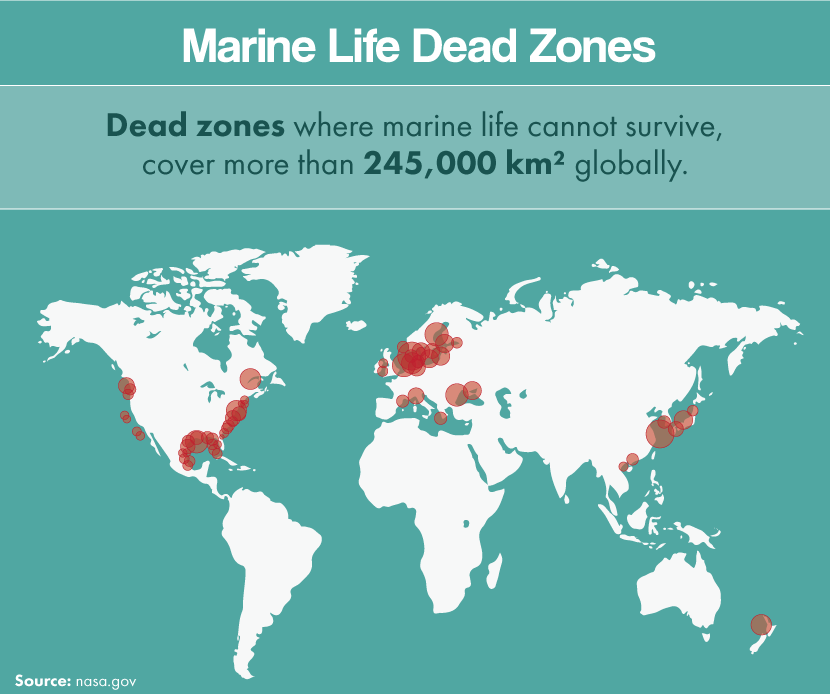
\includegraphics[width=200pt]{marine-life-dead-zones.png}
				\end{center}
				\caption{Répartition des zones mortes (source : nasa.gov)}
			\end{figure} \\
			Autre constat : certains pays dépassent en consommation la quantité d'eau renouvelable à disposition et exercent donc une pression sur le cycle de l'eau. \\
			La multitude de problématiques présentées ci-dessus explique pourquoi l'eau est au coeur des SDGs. Depuis de très nombreuses années, une attention particulière est portée à la qualité de l'eau et aux dangers liés à une contamination de celle-ci \cite{ashbolt_microbial_2004}. Le manque d'infrastructures sanitaires dans les régions en développement les rends vulnérables aux morts par contamination de l'eau. Neuf morts sur dix touchent les enfants, et tous les décès surviennent dans ces régions. \\
			Aujourd'hui, de nombreux outils permettent de suivre avec précision les indicateurs classiques de qualité de l'eau tels que le taux d'oxygène, l'acidité, la température, la conductivité etc. Ceci est très important pour la réalisation du but 6.3 : <<By 2030, improve water quality by reducing pollution, eliminating dumping and minimizing release of hazardous chemicals and materials, halving the proportion of untreated wastewater and substantially increasing recycling and safe reuse globally>> \cite{united_nations_goal_nodate-4}. \\
		
		\subsection{Bio-indicateurs}
			Depuis les années 1970, les auteurs de diverses études analysent les relations entre la faune et la qualité environnementale de leurs habitats. On considère en effet que les relevés sont capables de fournir des indicateurs sur l'état et la qualité de l'écosystème aquatique étudié. Dès lors, on a mis au point de nombreux outils basés sur les macro-invertébrés benthiques a des fins de diagnostiques concernant la qualité des écosystèmes aquatiques.\\
			En Europe, les macro-invertébrés benthiques sont les éléments les plus utilisés pour comprendre, analyser et révéler les pressions anthropiques exercées car ils présentent les caractéristiques suivantes :
			\begin{itemize}
				\item Ils sontrelativement sédentaires et certains sont extrêment sensibles ou résistants aux perturbations et pollutions importantes.
				\item Ils sont très hétérogènes, la plupart du temps abondants et disposent d'une grande variété de formes et d'espèces.
				\item Pour une variation environnementale donnée, il est très probable de trouver quelques organismes qui réagissent fortement et, souvent, de façon extrêmement rapide.
				\item La différence de caractéristiques entre les différents organismes va modifier leur réponse en fonction de la nature et de l'intensité du stress.
				\item Leur durée de vie qui varie de quelques mois à quelques années est suffisante pour enregistrer et surveiller la qualité environnementale.
				\item On peut trouver des macro-invertébrés benthiques de façon abondante dans tous les types d'habitats.
				\item Ils sont relativement aisés à collecter et présentent l'avantage, par rapport aux micro-organismes et au plancton, d'être bien plus facile à identifier.
			\end{itemize}
			L'IBGN est un des outils diagnistiques de la qualité des écosystèmes aquatiques qui utilise les macro-invertébrés benthiques pour leurs nombreuses caractéristiques. \\
			Le protocole de l'IBGN impose un échantillonage en 8 prélèvements réalisés sur des substrats différents, dans un ordre défini par la norme et en tenant compte de la vitesse du courant. On utilise un filet de type Surber d'une surface d' 1/20$^e$ de m$^2$ et donc les mailles mesurent 500$\mu$m. On calcule l'indice en estimant différents paramètres en utilisant une liste finie de 152 taxons. Parmi ces 152 taxons, 38 seront considérés comme indicateurs et permettent la définition de 9 groupes faunistiques correspondant à leur pollusensibilité. Le calcul se fait alors en 3 étapes :
			\begin{enumerate}
				\item On détermine la "classe de variété taxonomique" (A) qui est égale au nombre de taxons récoltés sur les 152 potentiellement présents. Un taxon est considéré présent même s'il est représenté par un seul individu.
				\item On détermine le "groupe faunistique indicateur" (B) en ne prenant en compte que les taxons indicateurs. Il doit y avoir au moins 3 individus (ou 10 pour certains taxons) par échantillon.
				\item L'indice est obtenu par la formule suivante : $A + (B - 1)$ avec $IBGN \le 20$
			\end{enumerate}
			\begin{figure}
				\begin{center}
					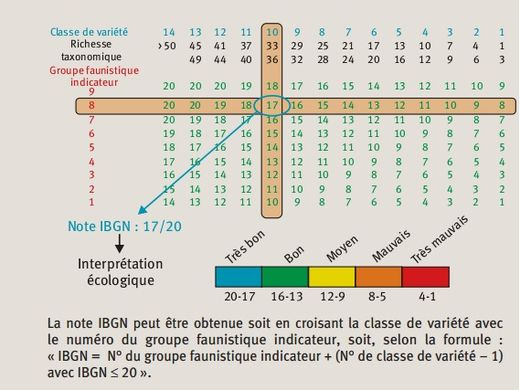
\includegraphics[width=300pt]{ibgn.jpg}
				\end{center}
				\caption{Calcul de l'IBGN (source : \cite{ibgn})}
			\end{figure}
			L'intérêt de cette méthode réside dans le fait qu'elle tient compte de toutes les communautés d'invertebrés et non pas uniquement des groupes les plus sensibles. Il est relativement aisé de récolter, manipuler et exploiter les informations. De plus, il est adapté au suivi de la qualité écologique d'un point d'eau de part ses larges possibilités d'applications. Le protocole permet de suivre spatialement les variations et perturbations, d'en suivre l'évolution à travers le temps ou de considérer le point d'eau isolément.
			Cependant, cette méthode d'analyse n'est pas adaptée aux zones sources et/ou profondes et ne permet pas d'évaluer la variabilité saisonnière liée aux cycles biologiques. Il n'est pas possible non plus d'identifier la nature exacte de la perturbation observée. De plus, certaines zones comme les rivières de haute montagne dont la diversité naturelle est faible on un indice inférieur à l'indice de référence ($IBGN = 20$) en dehors de toute perturbation. Pour les cours d'eau profonds, on préfère utiliser l'indice IBGA qui modifie légèrement le protocole de prélèvement en en effectuant certains par draguage. Lorsqu'il n'est pas possible d'effectuer un draguage (fonds encombrés et/ou navigation trop importante) on utilise la méthode IQBP qui consiste à laisser un piège à benthiques 1 mois au fond de l'eau pour que ceux-ci le colonisent. Les indices IBGA et IQBP sont également basés sur une note sur 20 établie sur l'analyse de la faune benthique.
		
		\subsection{Air}
			La qualité de l'air est aujourd'hui responsable de nombreuses maladies, cancers et décès. Une étude chinoise récente met en avant l'augmentation de la fréquence de visite des hopitaux pour des problèmes respiratoires lors de l'augmentation du nombre de particules fines dans l'air \cite{liu_effects_2016}. La réduction du nombre de morts attribuables à la qualité de l'air est un des indicateurs de l'objectif 3 (Good-Health and Well-Being) \cite{united_nations_goal_nodate-5}. En opposition à la qualité de l'eau, celle de l'air s'est dégradée lors de la dernière décennie. En 2012, la pollution de l'air est responsable d'environ 5.5 milions de morts à travers le monde et environ la moitié de la population mondiale est exposée à un air dont la concentration en particules fines est supérieure à 10 microgrammes/m$^{3}$ \cite{yale_university_epi_2016}. Certains chercheurs affirment aussi qu'on peut constater un lien entre le nombre de tumeurs malignes du cerveau dans une région géographique et son taux de particules fines \cite{andersen_long-term_nodate}. \\
			La pollution de l'air impacte également le changement climatique en modifiant la composition de l'atmosphère et des océans. L'augmentation de la quantité de CO$_{2}$ dans l'air influe sur l'acidité des océans et impacte donc les espèces marines sensibles à ces changements. La modification de la composition chimique des océans impacte directement la reproduction de certaines espèces marines et la capacité des espèces de cnidères, tels que les coraux, à créer leur exosquelette \cite{hoegh-guldberg_coral_2007}.  \\
	
	%\section{Monitoring sociétal}
	%	\subsubsection{Santé}
	%	\subsubsection{Sécurité}
	%	\subsubsection{Développement}
		
\section{Participation citoyenne}
	Les citoyens peuvent contribuer à la réalisation de ces SDGs par plusieurs moyens, qu'il s'agisse de la récupération, du traitement des données receuillies sur le terrain, de la mise à disposition de ressources ou d'outils. On peut citer en exemple le "World Water Monitoring Day", journée lors de laquelle des miliers de citoyens vont récupérer, dans les points d'eau proche de chez eux, des échantillonsdont la qualité est analysée. \\
	Lorsque l'étendue géographique à couvrir et/ou la durée des observations dans le temps sont des paramètres importants, il est intéressant de recourir à un nombre important de citoyens bénévoles non spécialistes plutôt qu'à un petit groupe d'expert. De plus, leur nombre et leur répartition sur le terrain permettent de limiter les risques financiers, de biais et d'évaluation non-neutre. Des protocoles standardisés sont nécessaires dans cette approche citoyenne.	

	\subsection{Projets}
		\subsubsection{Public Lab}
		Public Lab est un réseau américain de sciences citoyennes. Ils développent du matériel et des logiciels qui sont ensuite utilisés dans des projets de sciences citoyennes. Ils sont à l'origine de nombreux projets tels que l'Open Water Project, Open Air, Open Land, etc. et contribuent à d'autres tel que l'InfoAmazonia en participant à l'élaboration des composants utilisés dans le capteur Mae d'Agua.\\
			Public Lab a créé de nombreux capteurs spécialisés dans l'analyse des données environnementales. Le Riffle est designé pour être étanche, open source, open hardware et compatible avec un Arduino. Il permet initialement de mesurer la température de l'eau, mais il est également modulable et on peut lui ajouter des capteurs de turbidité, de pression et de conductivité. Cette modularité et son prix relativement bas lui offre une large variété de cas d'utilisation. Le Riffle est pensé pour répondre aux critères suivants :
			\begin{itemize}
				\item Faible consommation de batterie : le capteur doit pouvoir fonctionner au moins une semaine sans être rechargé.
				\item Du matériel libre : pour permettre à la communauté de le modifier et en faciliant l'ajout de nouveaux capteurs.
				\item Des logiciels libres : qui ont pour but de faciliter le transfert et la visualisation d'informations.
				\item Matériel de stockage libre : pour que les données de sorties soient au format CSV et sur une carte SD.
				\item Du matériel accessible : il doit être facile de remplacer un composant, et si possible de le trouver localement. Le tout doit pouvoir être encapsulé dans un conteneur étanche.
				\item Créer une communauté : en engageant des citoyens autour de la création d'un tel objet.
			\end{itemize}
			Le plus grand challenge est de trouver un conteneur étanche qui permette la réalisation des relevés désirés. Plusieurs approches plus ou moins satisfaisante sont proposées, mais la plus intéressante propose d'utiliser de simples bouteilles en plastique dont on perce le bouchon pour laisser sortir les capteurs.
			\begin{figure}
				\begin{center}
					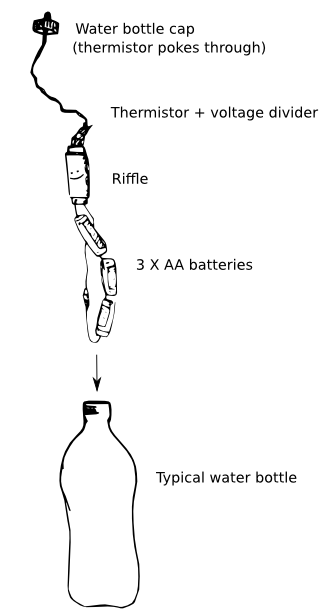
\includegraphics[width=100pt]{bottle_enclosure.png}
				\end{center}
				\caption{Idée générale de l'encapsulation du Riffle, de son alimentation en électricité et ddes différents capteurs (source : Public Lab)}
			\end{figure}
			Cette configuration a donné lieu à de nombreuses propositions comme l'utilisation de riz pour absorber les éventuelles fuites, ou encore l'ajout de capteurs de conductivité (qui n'étaient pas prévus dans le design initial). Il existe également des plans d'impression 3D pour imprimer un conteneur étanche.\\
			La carte possédant le circuit électronique a été développée pour être entièrement compatible avec l'IDE d'Arduino et d'une size qui lui permette de passer dans la plupart des goulots des bouteilles de 20mm. Le fait de devoir glisser le tout par l'embouchure demande également à ce que les broches de connexion se trouvent aux extrêmités de la carte afin que les cables passent verticalement.
			\begin{figure}
				\begin{center}
					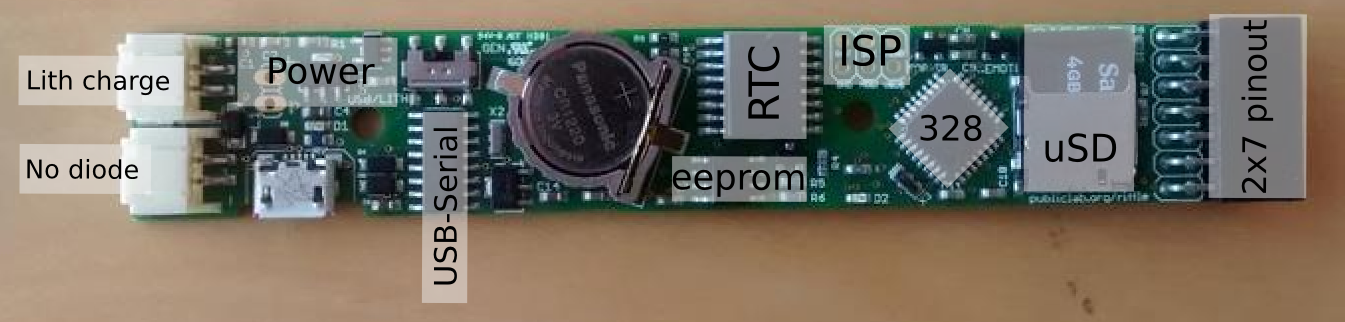
\includegraphics[width=300pt]{riffle_parts_2.png}
				\end{center}
				\caption{Dernière version du Riffle (source : Public Lab)}
			\end{figure}
			La configuration du Riffle est hautement modulable et permet par exemple l'ajout d'une carte GSM ou d'un émetteur/récepteur radio pour les télécommunications.  Le problème d'une carte SIM étant bien sûr les coûts mensuels liés à son utilisation. A noter que les télécommunications ont également un effet non négligeable sur la durée de vie d'un appareil. Les interfaces utilisées sont sélectionnées pour être compatibles avec la plus large variété de protocoles et de matériel électroniques externes. Les données recueillies sont ensuite fournies au format CSV ou TSV et c'est à l'utilisateur de voir comment il veut les traiter. Cette décision a été prise après discussion avec de nombreux hydrologues car il existe de nombreux workflows différents. Il est donc plus pertinent de présenter les données sous un format générique et de laisser le soin de les rendre compatible avec son propre système à l'utilisateur.\\
			Public Lab a également contribué à d'autres projets comme le Thermal Fish Bob (capteur de température basé sur la lumière), le Coqui qui peut émettre des fréquences de son audibles et effectuer des mesures de conductivité, de température et de visibilité, ou le Kit Initiative qui vise à mettre à disposition et distribuer les kits nécessaires aux différents challenges rencontrés.
		
		\subsubsection{InfoAmazonia}
			InfoAmazonia regroupe de nombreux projets autour de la forêt tropicale amazonienne. Les informations recueillies par sont ensuite rendues disponibles via une carte interactive. Celle-ci présente différentes vues, telles que, entre autres, les zones protégées, les zones de minages ou encore de déforestation. Les citoyens ayant des informations à diffuser sont invités à contribuer au projet au moyen d'un formulaire qui permet de soumettre sa propre histoire ou des données. Le projet InfoAmazonia est soutenu par plusieurs acteurs locaux. \\
			\begin{figure}
				\begin{center}
					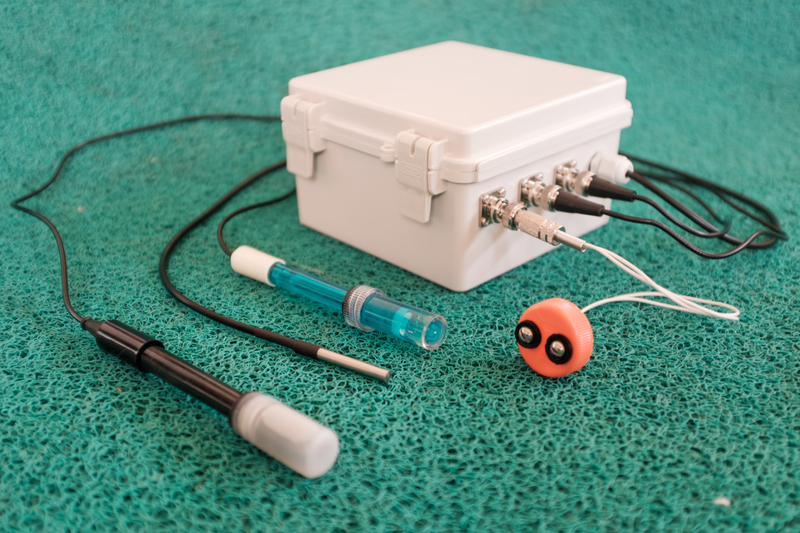
\includegraphics[width=300pt]{mae-dagua.jpg}
				\end{center}
				\caption{Mae d'Agua (source : Public Lab)}
			\end{figure}
			Parmi les différentes sources de données du projet, on peut notamment citer Mae d'Agua, un matériel ouvert qui permet de surveiller la qualité de l'eau. un réseau de capteurs sans fils (WSN) qui récupère les informations relatives à la qualité de l'eau telles que la conductivité électrique, le pH, le potentiel d'oxyréduction (OPR), la température, la pression barométrique ainsi que la température du capteur. Cet équipement peut être utilisé pour surveiller la qualité de l'eau dans des boîtes à eau, des citernes et réservoirs ainsi que les corps d'eau à faible débit. Inspiré du capteur "Riffle", ce matériel a été développé en collaboration avec Public Lab (réseau américain de science citoyenne) ainsi que Dev Technologia, une startup de Sao Paulo University. Les données recueillies sont envoyées à un serveur via le réseau de téléphonie mobile. Les relevés sont effectués à une fréquence d'un par heure. Il est nécessaire de nettoyer régulièrement les capteurs afin d'éviter que les relevés ne soient erronés à cause de l'accumulation de débris. Il s'agit d'un projet open source et open hardware, les fichiers et firmware sont disponible sous licence MIT. \\
			L'équipement est modulaire et comporte 3 modules :\\
			\begin{enumerate}
				\item Le premier module est un Arduino Mega. Il gère le traitement des données ainsi que l'alimentation en énergie depuis une source externe.
				\item Le deuxième module est une coque Arduino conçue grâce à la plateforme Eagle. Cette coque dispose d'un capteur de pression barométrique et de connecteurs permettant d'ajouter les capteurs de pH, température, OPR et de conductivité. Cette conception modulaire permet d'optimiser le rapport coût-bénéfices en fonction de l'application projetée.
				\item Le troisième module permet la communication au travers du réseau téléphonique mobile pour envoyer les données au serveur.
			\end{enumerate}
			Le projet est soutenu par Google et par des institutions et entreprises locales.

		\subsubsection{Reef Citizen Science Alliance}
			Ce projet regroupe des citoyens qui aident à collecter des données sur la grande barrière de corail, en Australie. Les volontaires peuvent participer à des ateliers de formation qui s'adressent aux personnes ayant des connaissances faibles ou modérées sur les coraux. Ils apprennent comment effectuer les relevés de façon simple. Il existe de nombreuses façon de contribuer sans effectuer cette formation, par exemple en signalant des espèces marines particulières lors d'une session de plongée ou de snorking au moyen d'une application pour smartphone. L'application permet également de signaler des évènements en temps réel et de voir ce que les volontaires peuvent faire autour d'eux pour contribuer. \\
			Les résultats de ces relevés sont largement utilisés par la Great Barrier Reef Foundation qui contribue à financer de nombreux projets de préservation et de  restauration de la barrière de corail Australienne.
		
		\subsubsection{World Water Monitoring Challenge}
			Le WWMC est un projet de EarthEcho International. Cet évènement, conduit chaque année entre mars et décembre, réunit plus de 1'500'00 participants dans un total de 146 pays. L'idée est d'équiper et former les citoyens afin qu'ils surveillent leurs points d'eau locaux tout autour du monde avec pour le moment 77'685 endroits surveillés. La sensibilisation et l'incitation à la surveillance pour protéger les ressources hydriques sont les points clés de ce projet. \\
			Les citoyens participent par plusieurs voies :
			\begin{itemize}
				\item Par la surveillance des points d'eau à l'aide de kits.
				\item Par le partage des données au travers d'une plateforme et des réseaux sociaux.
				\item Par l'utilisation des informations pour protéger les ressources hydriques vulnérables. 
			\end{itemize}
			Les kits comprennent : 1 livre d'instruction, 1 récipient pour les échantillons, 1 tube de à essais de pH, 1 fiole de d'oxygène dissous, 2 bandes de température, 50 comprimés de réactif au pH, 100 comprimés de réactif d'oxygène dissous, 1 disque de Secchi et 1 nuancier pour l'interprétation des résultats (DO, pH, turbidité). Les kits sont conçus pour permettre d'effectuer 50 tests et coûtent environ 50 dollars. Le projet permet également à certaines organisations, sous conditions, d'obtenir gratuitement des kits.
		
		\subsubsection{Riverfly Monitoring Initiative}
			Ce projet, réalisé aux Royaumes-Unis, réunis de nombreux acteurs tels que pêcheurs, authorités compétentes comme le ministère de l'environnement, scientifiques et entomologistes dans le but de protéger la qualité de l'eau des rivières, de mieux comprendre les populations des mouches de rivière et de conserver leur habitats. Ces insectes jouent un rôle fondamental dans les rivières, en particulier concernant l'alimentation de certains poissons et chauves-souris car ils font partie du plancton aérien. Ces insectes, apparus au Carbonifère (il y a environ 300 millions d'années) sont extrêmement sensibles à la pollution lumineuse et chimique, notamment par les pesticides. On compte parmi ces espèces les éphémères, les plécoptères et les trichoptères. Ils passent la plus grande partie de leur vie au stade larvaire, dans l'eau. De ce fait, les facteurs tels que le débit d'eau, sa qualité ou encore son niveau ont un impact majeur sur ces espèces. Leurs caractéristiques les rendent particulièrement pertinentes en tant qu'indicateurs lors d'études de la qualité de l'eau. Par exemple, lors du rejet d'eaux usées, un des bio-indicateurs de pollution peut être les populations de certaines espèces de plécoptères puisque celles-ci, sensibles à la quantité d'oxygène dissous, vont chuter brusquement. \\
			Le Riverfly Partnership organise des journées de formation pour les clubs de pêche et autres groupes de personnes concernées par la surveillance des cours d'eau. Les pêcheurs disposent d'une position privilégiée pour surveiller la qualité et l'état des cours d'eau dans lesquels ils pêchent. Ils sont nombreux a exprimer un intérêt à pouvoir eux-même effectuer les vérifications de l'eau. Les conditions pour participer à la RMI est d'avoir une personne prête à devenir coordinatrice locale ainsi que des membres prêts à suivre la journée des ateliers de formation qui consistent en diverses présentation et démonstrations pratiques de l'utilisation du matériel. 
			Ce projet préconise une fréquence de relevés mensuelle, ce qui rend les mesures sensibles aux fluctuations saisonnières et aux cycles naturels. On estime à une heure le temps nécessaire par volontaire pour effectuer les prélèvements. Les kits de prélèvement contiennent : un filet de 25cm (maille de 1mm), un grand plateau, un seau, un bac diviseur en 8 parties, une pipette, une loupe, une petite cuillère, un pinceau et le guide pratique de l'utilisation du matériel.\\
			Les résultats sont disponibles librement sur leur site web et permettent de visualiser au moyen d'une carte les endroits ou sont effectués les relevés. Ces données sont également partagées aux différents organismes gouvernementaux en charge de la protection et de la restauration de  l'environnement.
		
		\subsubsection{Restoration Assessment Initiative}
			La multitude de projets de monitoring de la qualité de l'eau a permit de démocratiser la participation citoyenne aux projets de surveillance locaux, notamment sur la détection de la pollution sur de larges périodes de temps. Bien que les différents acteurs des initiatives partagent un but commun, à savoir améliorer la qualité de l'eau, les conditions de pêche à la ligne et la biodiversité, il n'existe à ce jour aucun projet citoyen visant à évaluer le succès de la restauration qui vise à atteindre les buts énoncés ci-dessus. La Restoration Assessment Initiative propose un modèle standardisé pour évaluer la réponse biotique aux projets de restauration de l'environnement. Le but est de permettre la mise en place d'une base de donnée à large échelle permettant de connaître, à terme, les plus gros facteurs de succès et d'échecs des projets de restauration. Nos socitétés sont fortement influencées par les services que nous fournit l'écosystème, c'est pourquoi il est important de rétablir l'intégrité des cours d'eau et de stoper le déclin des espèces. Cela pose cependant un nombre non négligeable de challenges.
			Dans les zones dégradées, l'un des principaux problème est le manque de diversité des habitats. Cette donnée est critique puisqu'elle va contraindre la capacité d'un écosystème à se rétablir. En augmentant l'hétérogénéité des habitats, on aide à restaurer la biodiversité et l'intégrité de l'écosystème. Cette théorie n'a cependant pas beaucoup de preuves : les améliorations locales sont souvent surpassées par les études à large échelle et, à cause du manque de ressources, de temps et d'argent, 90\% des projets de restauration ne sont pas surveillés (USA, Australie, Europe) autrement que par une évaluation visuelle. Ces causes pourraient être mitigées par l'utilisation de sciences citoyennes en utilisant des protocoles standardisés de surveillance et des méthodes de mesures quantitatives pour mesurer les critères appropriés. Déployé à large échelle, cette approche offrirait une toute nouvelle perspective avec un coût relativement faible grâce aux avantages précités des sciences citoyennes.\\
			\begin{figure}
				\begin{center}
					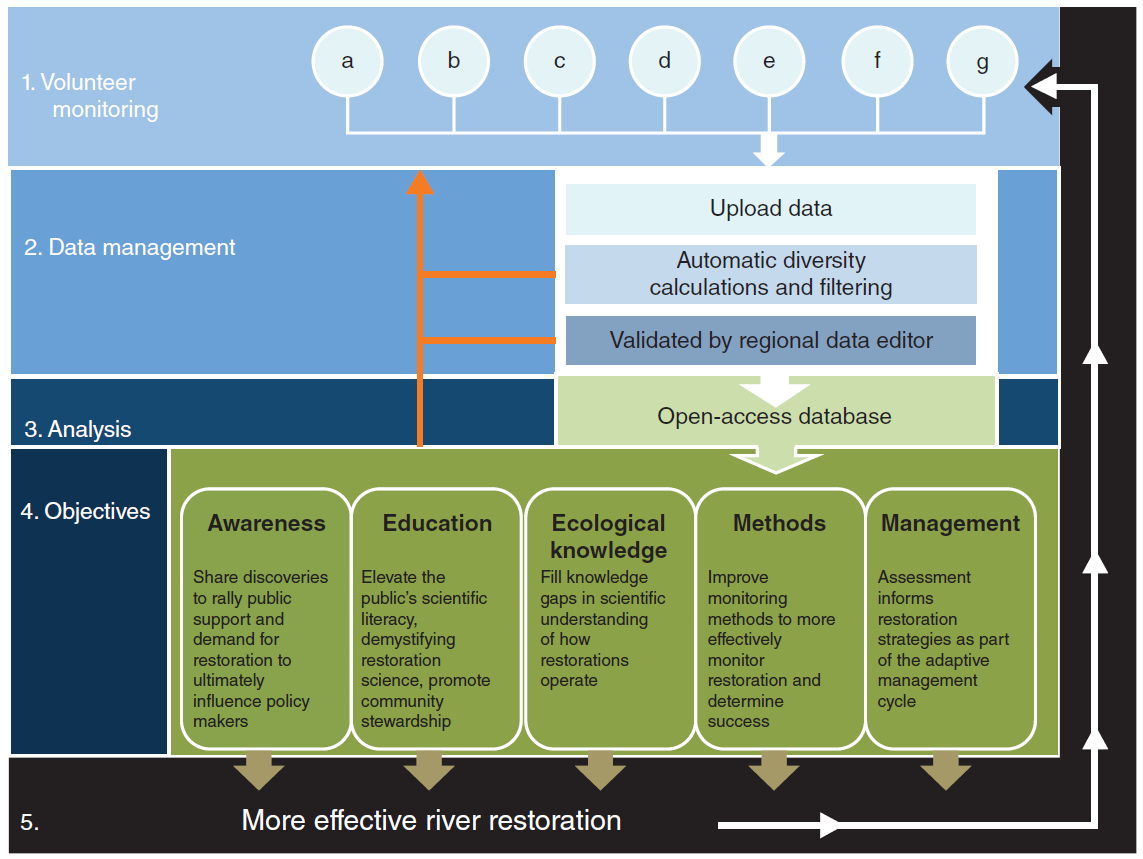
\includegraphics[width=300pt]{RAI.png}
				\end{center}
				\caption{RAI framework (source : \cite{hudart})}
			\end{figure}
			Les projets de restauration seraient ainsi plus personnalisés et les différents résultats, qu'ils soient positifs ou négatifs, seraient utilisés dans un but de guider les efforts et la recherche.
			Le RAI prend la Riverfly Monitoring Initiative en modèle mais ajoute l'analyse statistique Before-After Control-Impact (BACI) pour contrôler un point à la fois dans le temps et l'espace. L'anlyse BACI rend les données robustes puisqu'elle permet de distinguer les effets de la restauration et ceux des fluctuations saisonnières. L'étude doit cependant être menée sur plusieurs années puisque les prélèvements ne se font plus mensuellement mais annuellement. Les mesures effectuées sont plus nombreuses et le nombre de taxons évalués est plus grand. La différence fondamentale entre le modèle proposé et l'approche de la RMI est que les données sont aggrégées pour comprendre les causes de succès ou d'échecs des projets de restauration. Ceci permet d'investir les ressources pour influencer positivement les futurs projets et de compléter la base de données au fur et à mesure de l'évolution des projets.
		
		\subsubsection{Autres projets, logiciels et applications}
			Les citoyens volontaire peuvent également contribuer à des projets de sciences citoyennes par le biais d'applications comme Epicollect, INaturalist, Water Reporter, Project Noah, NatureBytes etc.
		
		\subsubsection{Open Air}
		\subsubsection{etc...}
				INatrualist, NatureBytes, Epicollect, SeeClickFix, Water Reporter, Project Noah	

\section{Conclusion}\label{sec:conclusion}

% use section* for acknowledgement
\section*{Remerciements}


\bibliographystyle{alpha}
\bibliography{soa} %%% soa.bib is the file containing bibliographic entries


% that's all folks
\end{document}


